\chapter{Theoretical Background}

This chapter will give a brief overview about the underlying theoretical background in the fields of antenna theory, spatial sampling and will some methods to derive the \ac{TRP} out of spherical measurements.

\section{Antenna Field Regions}
\begin{figure}[H]
\centering
\def\svgwidth{0.6\textwidth}
\input{Bilder/AntennaApature.pdf_tex}
\caption{An arbitrary radiating aperture in the $xy$ plane. \cite{7942128}}
\label{arbaperturexy}
\end{figure}

\ac{FF}-distance and \ac{NF}-distance are derivable from the phase fluctuation due to the maximum diameter of the antennas aperture \cite{7942128} in a distance $R$ from the antennas phase center. The phase fluctuation is given by the different length of $r$ and $R$, as you can see in figure \ref{arbaperturexy}. The maximum runtime difference is found at the minimum radius of the circle enclosing the aperture at $\sfrac{D}{2}$. The field boundaries are derived from the Taylor series of the function of the phase in dot $P$. \cite{7942128}


\subsection{Near-Field}

The reactive \acf{NF} is according to \cite{balanis} \glqq that portion of the near-field region immediately surrounding the antenna wherein the reactive field predominates.\grqq{ }The Boundary of that field region is derived for big apertures by a line source and the underlying phase fluctuation of  $\Delta\phi = \sfrac{\pi}{8} \ \widehat{=}\  22.5^\circ$. The boundary is \cite{8393926}:
\begin{equation}
r_{\text{NF}} = 0.62\sqrt{\frac{D^3}{\lambda}}
\end{equation}
After that the radiating \ac{NF} (Fresnel) -region follows, which is defined as \glqq that region of the field of an antenna between the reactive near-field region and the far-field region wherein radiation fields predominate and wherein the angular field distribution is dependent upon the distance from the antenna.\grqq

\subsection{Far-Field}

The fraunhofer distance is derived from optical considerations. The commonly used terminology is \acf{FF}-Distance. According to \cite{balanis} the \ac{FF}-distance is \glqq that region of the field of an antenna where the angular field distribution is essentially independent of the distance from the antenna.\grqq \\
The amount of independency is derived from the phase fluctuation in the distance $r_{\text{FF}}$ \cite{19510}:

\begin{equation}
\Delta\phi = \frac{\pi D^2}{4\lambda\cdot r_{\text{FF}}} ,\ D\gg\lambda 
\end{equation}

The commonly used maximum phase fluctuation is $\Delta\phi = \sfrac{\pi}{8} \ \widehat{=}\  22.5^\circ$. With that the well known formula
\begin{equation}
r_{\text{FF}} = \frac{2D^2}{\lambda}
\end{equation}

can be derived.

\subsection{Derat Distance}

The Derat distance is that distance, in which the main beam of an antenna is in \ac{FF} condition. For the understanding of the Derat distance $r_{\text{Dr}}$ other considerations need to take place: It is about spherical modes described by spherical Hankel functions  of the second kind. \cite{8393926} \cite{hansen}\\
In \cite{8393926} it is shown, that higher order modes than 

\begin{equation}
N = \lceil 1.0252\cdot\left(\frac{\pi D}{\lambda}\right)^{0.8633} \rceil
\end{equation}

have a maximum influence to the \ac{EIRP} of $\SI{0.5}{\decibel}$. With that the Derat distance can be derived to:

\begin{equation}
r_{\text{Dr}} = \lambda\left(\frac{\pi D}{\lambda}\right)^{0.8633}\left(0.1673\left(\frac{\pi D}{\lambda}\right)^{0.8633}+0.1632\right)
\end{equation}

\subsection{Example: Standard Gain Horn}

\begin{figure}[H]
\centering
  \centering
  \subfigure[Wave impedance]{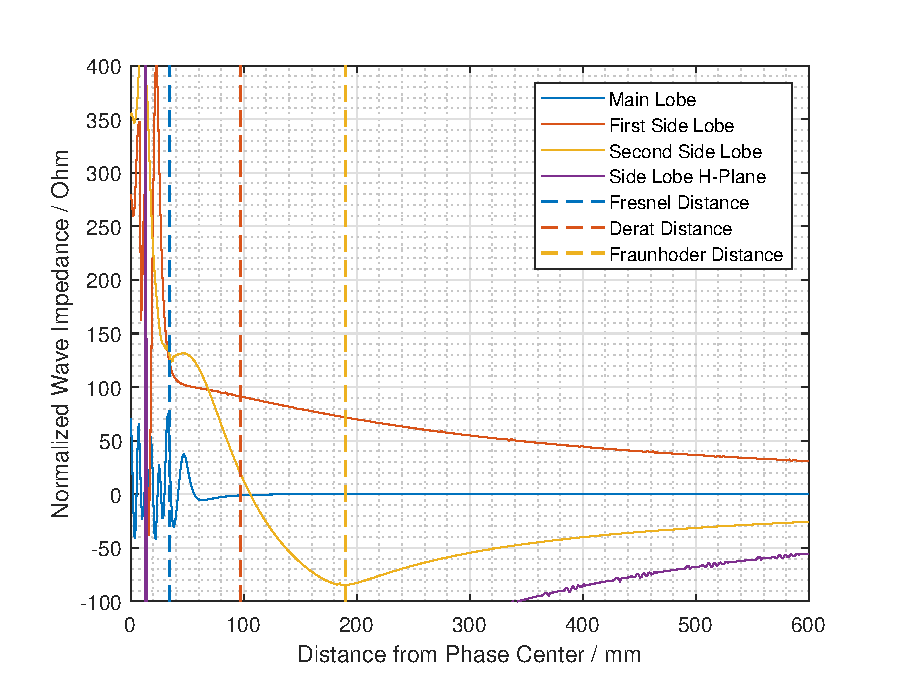
\includegraphics[width=0.49\textwidth]{Matlab/NormWaveImpHorn.eps}}
  \centering
  \subfigure[Phase]{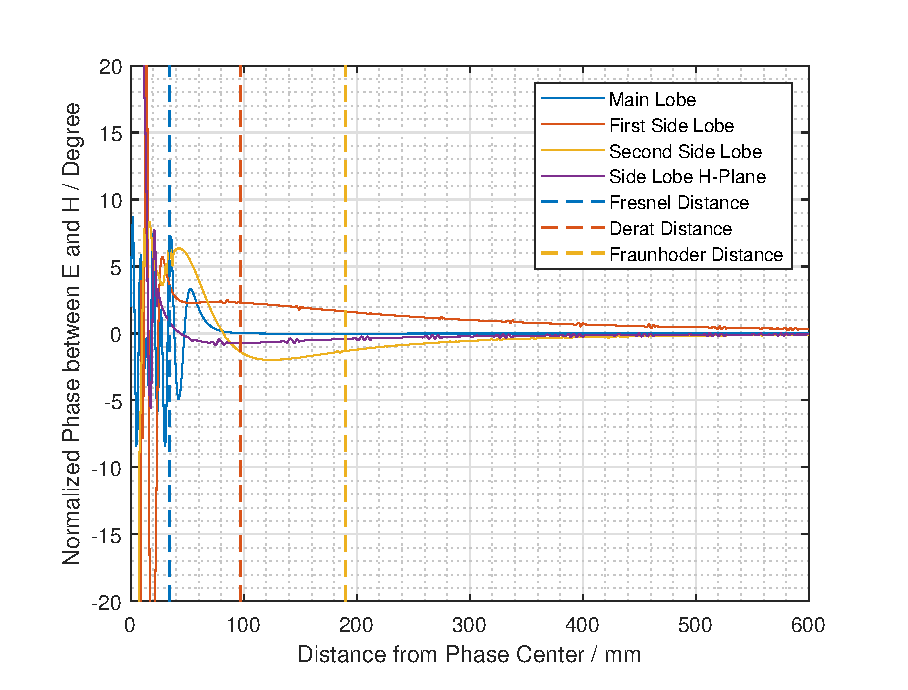
\includegraphics[width=0.49\textwidth]{Matlab/NormPhaseHorn.eps}}
  \centering
  \subfigure[Antenna Pattern E-Plane]{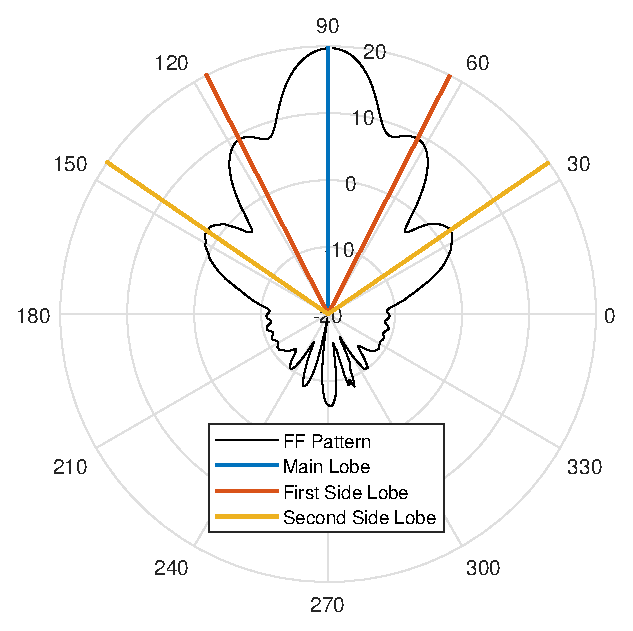
\includegraphics[width=0.3\textwidth]{Matlab/ePlanePattern.eps}}
\caption{Beam comparison of a $\SI{20}{\decibel}$ \ac{SGH} at $\SI{28}{\giga\hertz}$}
\label{fig:beamcpmp}
\end{figure}

To clarify the introduced distances they will be proofed based on a $\SI{20}{\decibel}$ \ac{SGH} at $\SI{28}{\giga\hertz}$. If you look in the annex at figure \ref{fig:fielddist} you see the front view of this horn with the underlying field distribution. The polarisation is in $y$-direction, so the $yz$-plane is called E-plane and the $xz$-plane is called H-plane from here on.\\
In figure \ref{fig:beamcpmp} the normalized wave impedance (a) and the normalized phase between E- and H-field components over the distance to the phase center are plotted. To clarify the designations the directions are plotted in (c). The data has been produces by CST\texttrademark , a full wave simulation tool. Complex data in $x$, $y$, and $z$ direction was exported to Matlab\texttrademark and there post processed.\\
Also the field boundaries from the sections above are plotted with dashed lines. For deriving the boundaries only the opening of the horn in the E-plane was taken to account. This is rational because the field distribution and thus the usage of the aperture is known, refer to figure \ref{fig:fielddist}. As you can see in the E-plane the aperture is fully used, if the H-plane would have been plotted and the field boundaries would be calculated the used opening would be shorter as the physical length of the horns aperture. But if the field distribution or the polarisation is unknown the smallest circle enclosing the aperture has to be taken.\\
The main lobe (blue line) is, as you can see in figure \ref{fig:beamcpmp}, from Derat-distance on in \ac{FF} condition because on the one hand side the wave impedance reached its endvalue of $\SI{377}{\ohm}$ and on the other hand E- and H-field are coherent.
Considering the side lobes it can be seen that in the reactive \ac{NF} the field conditions are very unstable, whereas the fields in the radiating \ac{NF} become more stable. In the \ac{FF} the field values are continually decreasing the offset from their final value.

\section{Spatial Sampling Approaches}

\subsection{Derivation of the Spatial Sampling considering the Array Factor}

\subsection{Constant Step}
Constant Step, Constant Step with swept Azimuth,

\subsection{Constant Density}

Constant Density

\subsection{Other}

Spiral Scan
Cardinal Cuts with or without Pattern Multiplication

\section{Total Radiated Power Integrals in Comparison}

\subsection{Sinus Theta}

\subsection{Jacobi}

\subsection{Clenshaw-Curtis}

\section{Measurement Distance}